\section{Исследование управляемости}

Рассмотрим систему $\dot{x} = Ax + Bu$, где 
\begin{equation}
    \begin{array}{ccc}
        A = \begin{bmatrix}
            0 & 4 & 2 \\
            -4 & -8 & -4 \\
            4 & 4 & 0
        \end{bmatrix}, &
        B = \begin{bmatrix}
            -3 \\
            -5 \\
            -2
        \end{bmatrix}, &
        x_1 = \begin{bmatrix}
            -4 & 0 & 0
        \end{bmatrix}
    \end{array}
\end{equation}

\subsection{Управляемость системы}
\subsubsection{Матрица управляемости}
Найдем матрицу управляемости $U = [B, AB, A^2B]$: 
\begin{equation}
    U = \begin{bmatrix} 
        \begin{array}{c|c|c}
            \begin{bmatrix}
                -3 \\
                5 \\
                -2
            \end{bmatrix} & 
            \begin{bmatrix}
                0 & 4 & 2 \\
                -4 & -8 & -4 \\
                4 & 4 & 0
            \end{bmatrix} \times 
            \begin{bmatrix}
                -3 \\
                5 \\
                -2
            \end{bmatrix} &
            \begin{bmatrix}
                0 & 4 & 2 \\
                -4 & -8 & -4 \\
                4 & 4 & 0
            \end{bmatrix}^2 \times
            \begin{bmatrix}
                -3 \\
                5 \\
                -2
            \end{bmatrix}
        \end{array}   
    \end{bmatrix}
\end{equation}
\begin{equation}
    U = \begin{bmatrix}
        -3 & 16 & -64 \\
        5 & -20 & 64 \\
        -2 & 8 & -16 \\
    \end{bmatrix}
\end{equation}

Определим ранг матрицы управляемости:
\begin{equation}
    \text{rank}(U) = 3
\end{equation}

Так как ранг матрицы управляемости равен порядку системы, то система является полностью управляемой согласно критерию Калмана.

\subsubsection{Управляемость собственных значений}
Найдем спектр матрицы $A$:
\begin{equation}
    \sigma(A) = \{-4, -2-2j, -2+2j\}
\end{equation}

Для каждого собственного значения найдем матрицу Хаутуса $H_i = \begin{bmatrix} A - \lambda_i I & B \end{bmatrix}$ и определим ее ранг:
\begin{enumerate}
    \item $\lambda_1 = -4$: $H_1 = \begin{bmatrix}
        4 & 4 & 2 & -3\\
        -4 & -4 & -4 & 5 \\
        4 & 4 & 4 & -2
    \end{bmatrix}$, $\text{rank}(H_1) = 3$, собственное значение управляемо.
    \item $\lambda_2 = -2-2j$: $H_2 = \begin{bmatrix}
        2+2j & 4 & 2 & -3\\
        -4 & -6+2j & -4 & 5 \\
        4 & 4 & 2+2j & -2
    \end{bmatrix}$, $\text{rank}(H_2) = 3$, собственное значение управляемо.
    \item $\lambda_3 = -2+2j$: $H_3 = \begin{bmatrix}
        2-2j & 4 & 2 & -3\\
        -4 & -6-2j & -4 & 5 \\
        4 & 4 & 2-2j & -2
    \end{bmatrix}$, $\text{rank}(H_3) = 3$, собственное значение управляемо.
\end{enumerate}
Каждое собственное значение матрицы $A$ является управляемым. 

\subsubsection{Диагональная форма системы}
Найдем диагональную форму системы, заменив базис на базис из собственных векторов матрицы $A$:
\begin{equation}
    \dot{\hat{x}} = P^{-1}AP\hat{x} + P^{-1}Bu
\end{equation}
Где $P$ -- матрица собственных векторов матрицы $A$. 
Найдем собственные векторы матрицы $A$:
\begin{equation}
    \begin{array}{ccc}
        v_1 = \begin{bmatrix} -1 \\ 1 \\ 0 \end{bmatrix} &
        v_2 = \begin{bmatrix} \frac{1}{2} - \frac{i}{2} \\ -1 \\ 1 \end{bmatrix} &
        v_3 = \begin{bmatrix} \frac{1}{2} + \frac{i}{2} \\ -1 \\ 1 \end{bmatrix} 
    \end{array}
\end{equation}
Тогда матрица $P$:
\begin{equation}
    P = \begin{bmatrix}
        -1 & \frac{1}{2} - \frac{i}{2} & \frac{1}{2} + \frac{i}{2} \\
        1 & -1 & -1 \\
        0 & 1 & 1
    \end{bmatrix}
\end{equation}
Система преобразуется к виду:
\begin{equation}
    \dot{\hat{x}} = \begin{bmatrix}
        -4 & 0 & 0 \\
        0 & -2-2j & 0 \\
        0 & 0 & -2+2j
    \end{bmatrix} \hat{x} + 
    \begin{bmatrix}
        3 \\
        -1 + j \\ 
        -1 - i
    \end{bmatrix} u
\end{equation}

Так как все элементы $P^{-1}B$ не равны нулю, то система является полностью управляемой.

\subsection{Грамиан управляемости}
Найдем грамиан управляемости $P(t_1)$:
\begin{equation}
    P(t_1) = \int_{0}^{t_1} e^{At}BB^Te^{A^Tt}dt
\end{equation}
Вычислим грамиан управляемости для $t_1 = 3$
\begin{equation}
    P(3) = \begin{bmatrix}
        0.79 & -1.45 & 0.61 \\ 
        -1.45 & 2.86 & -1.12 \\ 
        0.61 & -1.12 & 0.51 \\ 
    \end{bmatrix}
\end{equation}

Найдем собственные числа Грамиана управляемости: 
\begin{equation}
    \sigma(P(3)) = \{ 4.06, 0.02, 0.08 \}
\end{equation}
Все собственные числа Грамиана управляемости положительны, что говорит о том, что система является управляемой.


\subsection{Управление системой}
Найдем управление $u(t)$, которое будет переводить систему из состояния $x(0) = 0$ в состояние $x_1 = x(t_1) = \begin{bmatrix} -4 & 0 & 0 \end{bmatrix}^T$. 
\begin{equation}
    u(t) = B^Te^{A^T(t_1 - t)}P(t_1)^{-1}x_1
\end{equation}

\begin{figure}[H]
    \centering
    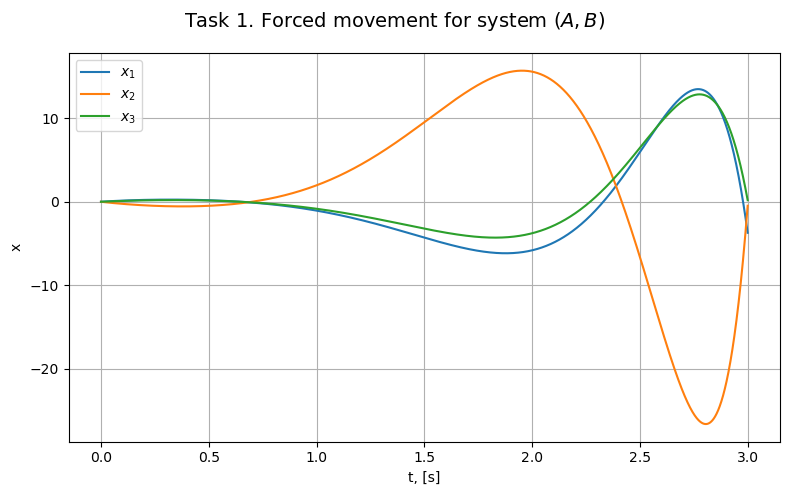
\includegraphics[width=\textwidth]{../../plots/task_1_1.png}
    \caption{Управление системой}
    \label{fig:task1_control_signal}
\end{figure}

\begin{figure}[H]
    \centering
    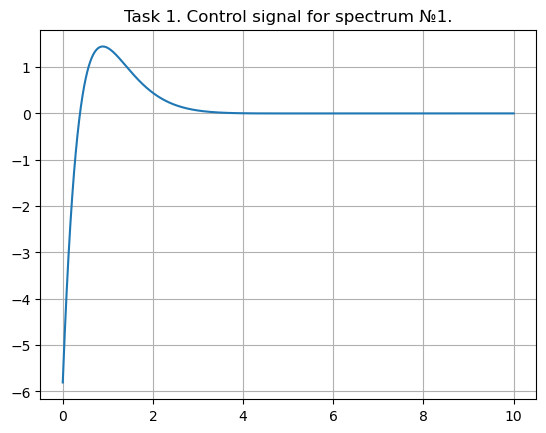
\includegraphics[width=0.9\textwidth]{../../plots/task_1_2.png}
    \caption{Состояние системы}
    \label{fig:task1_state}
\end{figure}

\subsection{Вывод}
В ходе исследования системы, представленной в данной задаче, 
было установлено, что она обладает свойством полной управляемости. 
Это подтверждено с использованием критерия Калмана, 
а также анализом управляемости собственных значений 
и диагональной формы системы. Дополнительно был вычислен 
грамиан управляемости, и проведена проверка его собственных чисел. 
Для проверки работоспособности управления было выполнено моделирование, 
в ходе которого система успешно переводилась в заданное состояние. 
Результаты моделирования подтвердили корректность работы управления 
и управляемость системы в целом.